\documentclass[12pt]{article}

% \usepackage[english]{babel}
\usepackage[brazilian]{babel}
\usepackage[letterpaper,top=2cm,bottom=2cm,left=3cm,right=3cm,marginparwidth=1.75cm]{geometry}

% Useful packages
\usepackage{amsmath}
\usepackage{graphicx}
% \usepackage[colorlinks=true,linkcolor=blue]{hyperref}
\usepackage{hyperref}
\usepackage{listings}
\usepackage[figure,table,lstlisting]{totalcount}
\usepackage{tcolorbox}
\usepackage{listings}
\usepackage{xcolor}
\usepackage{setspace}
\usepackage{float} 
\usepackage[numbers]{natbib}



\hypersetup{
    colorlinks=true,
    linkcolor=black,
    filecolor=magenta,      
    urlcolor=cyan,
    pdftitle={Trabalho pratico de projeto e analise de algoritmos},
    pdfpagemode=FullScreen,
    }

\definecolor{verde}{rgb}{0.25,0.5,0.35}
\definecolor{jpurple}{rgb}{0.5,0,0.35}

\lstset{
  language=C++,
  basicstyle=\ttfamily\small,
  keywordstyle=\color{jpurple}\bfseries,
  stringstyle=\color{red},
  commentstyle=\color{verde},
  morecomment=[s][\color{blue}]{/**}{*/},
  extendedchars=true,
  showspaces=false,
  showstringspaces=false,
  numbers=left,
  numberstyle=\tiny,
  breaklines=true,
  backgroundcolor=\color{cyan!10},
  breakautoindent=true,
  captionpos=b,
  xleftmargin=0pt,
  tabsize=4
}

\renewcommand{\lstlistingname}{Código}
\renewcommand{\lstlistlistingname}{Lista de Códigos Fonte}

\newcommand\conditionalLoF{%
    \iftotalfigures
        \listoffigures
    \fi}
\newcommand\conditionalLoT{%
    \iftotaltables
        \listoftables
    \fi}
\newcommand\conditionalLoL{%
    \iftotallstlistings
        \lstlistoflistings
    \fi}

\newcommand{\DESCRICAO}[1]{
    % set flexible interword space
    \setlength{\spaceskip}{0.5em plus 1em minus 0.1em}%
    % add some space with not as much flexibility, but only
    % if some space precedes
    \ifdim\lastskip>0pt \hspace{0.5em plus 0.5em minus 0.1em}\fi
    \texttt{\textbf{\color{red}#1}}
}

\newcommand{\CAPA}[4]{
    % 1) Título
    % 2)
    % 3)
    % 4)
    \begin{titlepage}
    	
    	  \vfill
    	
    	  \begin{center}
    	    \begin{large}
    	      Universidade Federal de Ouro Preto - UFOP
    	    \end{large}
    	  \end{center}
    	
    	  \begin{center}
    	    \begin{large}
    	      Instituto de Ciências Exatas e Biológicas - ICEB
    	    \end{large}
    	  \end{center}
    	
    	  \begin{center}
    	    \begin{large}
    	      Departamento de Computação - DECOM
    	    \end{large}
    	  \end{center}
          
          \begin{center}
    	    \begin{large}
              Ciência da Computação
    	    \end{large}
    	  \end{center}
    	  
    	  \vfill
          \vfill
    	
    	  \begin{center}
    	    \begin{Huge}
    	      #1\\
    	    \end{Huge}
    	    \begin{Large}
              #2\\
    	    \end{Large}
    	  \end{center}
    	  
    	  \vfill
    	  
    	  \begin{center}
    	    \begin{large}
              #3
    	    \end{large}
    	  \end{center}
    	
    	  \begin{center}
    	    \begin{large}
    	      Professor: #4
    	    \end{large}
    	  \end{center}
    	
    	  \vfill
          \vfill
    	
    	  \begin{center}
    	    \begin{large}
    	      Ouro Preto \\
    	      \today \\
    	    \end{large}
    	  \end{center}    
    
    
    \clearpage
    \newpage

    \tableofcontents
    \conditionalLoF
    \conditionalLoT
    \conditionalLoL
	
    % \thispagestyle{empty}
    % \tableofcontents
    % \newpage
    % \thispagestyle{empty}
    
    % \listoffigures
    
    % \lstlistoflistings
    % \newpage
    % \thispagestyle{empty}
    \end{titlepage}
}

\begin{document}
\onehalfspacing

\CAPA{Trabalho Prático}{BCC241 - Projeto de Análise de Algoritmos}{
Felipe Braz Marques - 22.1.4030
\linebreak 
Matheus Peixoto Ribeiro Vieira - 22.1.4104 
\linebreak 
Pedro Henrique Rabelo Leão de Oliveira - 22.1.4022 
}{Anderson Almeida Ferreira}


\section{Introdução}
    Neste trabalho, propõe-se a implementação de algoritmos que resolvem três diferentes problemas utilizando as técnicas de backtracking, branch and bound e redução. Os problemas abordados são: Satisfabilidade, Clique e Conjunto Independente. A Satisfabilidade, ou SAT, é um problema de grande importância prática, com aplicações em diversas áreas, como teste de circuitos e design de software. Um exemplo clássico de SAT é a busca por uma atribuição de valores de verdade para variáveis em uma fórmula booleana na forma normal conjuntiva (CNF). Além disso, como destacado por \citep{dasgupta2006algorithms}, os problemas de Clique e Conjunto Independente podem ser reduzidos um ao outro de maneira simples, pois um conjunto de nós que forma um Conjunto Independente em um grafo é equivalente a um conjunto que forma um Clique em seu grafo complementar. Dessa forma, a solução de um dos problemas pode ser obtida a partir do outro, facilitando o processo de implementação.
    
    
    A codificação foi feita em Python sem o uso de bibliotecas adicionais para a implementação dos algoritmos.

\subsection{Considerações iniciais}

Algumas ferramentas foram utilizadas durante a criação deste projeto:

\subsection{Ferramentas utilizadas}
Algumas ferramentas foram utilizadas para testar a implementação, como:
\begin{itemize}
    \item Linguagem utilizada: Python
    \item Biblioteca para exibição dos grafos: Matplotlib e networkx
\end{itemize}



\clearpage

\section{Clique}
    Para resolver o problema do Clique, onde o objetivo é encontrar um conjunto máximo de vértices tal que todas as possíveis arestas entre eles estejam presentes, foi utilizado uma solução Branch and Bound onde foram definidos os seguintes pontos do problema:
    \begin{itemize}
        \item \textbf{Variáveis para a solução:} \(X_1, \dots, X_n\), onde \(X_i\) representa um vértice pertencente ao grafo.
        \item \textbf{Domínio para as variáveis da solução:} \{0, 1\}, onde 0 indica que aquele vértice não faz parte do clique máximo e 1 indica o contrário.
        \item \textbf{Restrições:} Todos os vértices representados pelas variáveis que possuem valor 1 devem estar conectados entre si através de uma aresta.
        \item \textbf{Objetivo:} Obter o maior conjunto possível de vértices tal que todas as possíveis arestas entre eles estejam presentes.
    \end{itemize}

    \par Primeiro, o problema foi lido através de uma função e armazenado em uma variável na qual guarda o número de vértices do grafo e a matriz de adjacência do mesmo. 
    
    \par Depois, como melhor solução de início foi gerado um vetor através de uma função que varre a matriz de adjacência em busca de uma célula na qual indica que dois vértices estão conectados. Quando encontra, faz com que esse vetor tenha o valor 1 nas posições que representam esses respectivos vértices e valor 0 nas demais posições. Caso não encontre, o vetor terá apenas a primeira posição com o valor 1 e as demais com o valor 0, indicando um clique com apenas o primeiro vértice do grafo.
\begin{lstlisting}[caption={Função que gera a melhor solução inicialmente},label={lst:codClique1},language=Python]
def geraSolucao(problema):
    solucao = [0] * problema[0][0]

    for i in range(problema[0][0]):
        for j in range(problema[0][0]):
            if(problema[i+1][j] == 1):
                solucao[i] = 1
                solucao[j] = 1
                return solucao

    solucao[0] = 1
    return solucao
 \end{lstlisting}

    \par A solução inicial é um vetor com o número de posições igual ao número de vértices do grafo, com todas elas possuindo o valor -1, representando que as variáveis estão "livres", sem nenhum valor atribuído a elas, e, portanto, a solução inicial está vazia.

    \par Por fim, a função principal é chamada para encontrar a melhor solução, ou seja, o clique máximo, utilizando branch and bound como estratégia.
\begin{lstlisting}[caption={Função que encontra o clique máximo através de branch and bound},label={lst:codClique2},language=Python]
def branchAndBoundClique(solucao, i, problema, melhor):
    if eCompleta(solucao, problema):
        melhor[:] = solucao
        return melhor
    
    else:
        for j in range(2):
            solucao[i] = j
            
            if(eConsistente(solucao, problema, i) and ePromissora(solucao, problema, melhor, i)):
                melhor = branchAndBoundClique(solucao, i+1, problema, melhor)
            
            solucao[i] = -1
        
        return melhor
 \end{lstlisting}

     \par Para a verificar se a solução é completa, verifica-se se nenhuma posição do vetor solução possui o valor -1, o que significa que todas as variáveis tem valores 0 ou 1 atribuídos a elas.

     \par Já para verificar se uma solução é consistente, verifica-se, através da matriz de adjacência, se os vértices representados pelas variáveis que possuem valor 1 na solução possuem todas as possíveis arestas entre eles. Caso contrário, a solução é inconsistente e ocorre a poda daquele ramo.
\begin{lstlisting}[caption={Função que verifica a consistência da solução até o momento},label={lst:codClique3},language=Python]
def eConsistente(solucao, problema, i):
    verticesNaSolucao = []
    
    for j in range(i+1):
        if solucao[j] == 1:
            verticesNaSolucao.append(j)

    for j in range(len(verticesNaSolucao)-1):
        for k in range(j+1, len(verticesNaSolucao)):
            if(problema[verticesNaSolucao[j]+1][verticesNaSolucao[k]] == 0):
                return False
            
    return True 
 \end{lstlisting}

  \par Para a verificar se uma solução é promissora, adotamos a estratégia de somar o número de vértices com valor 1 no vetor da solução, ou seja, os vértices pertencentes ao clique até então, com o restante de posições do vetor sem valor atribuído, ou seja, com o valor -1. Dessa forma, obtemos o número máximo de vértices que estarão presentes naquela solução e, posteriormente, comparamos ele com o número de vértices do clique da melhor solução até o momento. Para obtermos esse último, apenas somamos os valores presentes nas variáveis da solução, uma vez que elas possuem valor 0 ou 1, e, portanto, a soma terá o valor do número de vértices presentes nesse clique.
\begin{lstlisting}[caption={Função que verifica se a solução até o momento é promissora},label={lst:codClique4},language=Python]
def ePromissora(solucao, problema, melhor, i):
    numVerticesMelhor = sum(melhor)
    numVerticesMaximoSolucao = 0 # armazena o numero maximo de vertices possiveis nessa solucao
    
    for j in range(i+1):
        numVerticesMaximoSolucao += solucao[j]

    numVerticesMaximoSolucao += (problema[0][0] - (i+1))
    
    return numVerticesMaximoSolucao > numVerticesMelhor
 \end{lstlisting}

\subsection{Exemplos de instância do problema}
    \subsubsection{Instância 1}
        \begin{tcolorbox}[title=Arquivo de entrada para a instância 1, width=\linewidth, 
          fontupper=\ttfamily, 
          halign=flush left]
            9 \\
            0 0 1 0 0 0 0 0 0 \\
            0 0 1 0 0 0 0 0 0 \\
            1 1 0 1 1 0 0 0 0 \\
            0 0 1 0 0 0 1 0 0 \\
            0 0 1 0 0 1 0 1 0 \\
            0 0 0 0 1 0 0 0 0 \\
            0 0 0 1 0 0 0 1 1 \\
            0 0 0 0 1 0 1 0 1 \\
            0 0 0 0 0 0 1 1 0 \\
        \end{tcolorbox}

        \begin{tcolorbox}[title=Saída da instância 1, width=\linewidth, 
          fontupper=\ttfamily, 
          halign=flush left]
            [0, 0, 0, 0, 0, 0, 1, 1, 1] \\
            Vértices presentes no clique: \\
            7 \\
            8 \\
            9 \\
            Tempo de execução: 0.001000 segundos \\
        \end{tcolorbox}

        \begin{figure}[H]
            \centering
            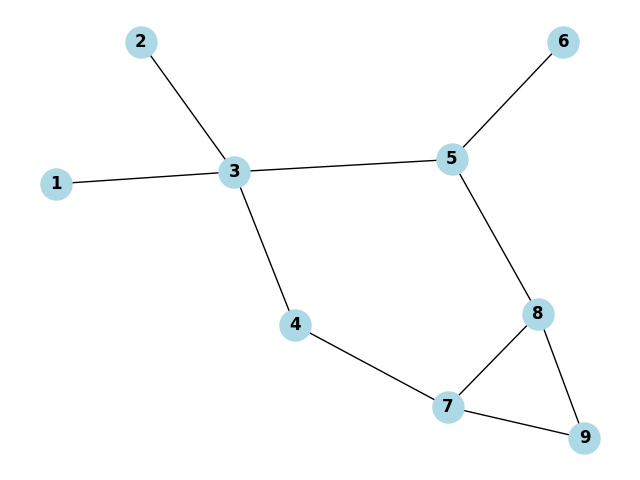
\includegraphics[width=0.65\textwidth]{grafo_instancia1.png}
            \caption{Grafo da instância 1 de entrada.}
            \label{fig:instancia1}
        \end{figure}

    \subsubsection{Instância 2}
        \begin{tcolorbox}[title=Arquivo de entrada para a instância 2, width=\linewidth, 
          fontupper=\ttfamily, 
          halign=flush left]
            5 \\
            0 1 1 1 0 \\
            1 0 0 0 0 \\
            0 1 0 1 1 \\
            1 0 1 0 1 \\
            0 0 1 1 0 \\
        \end{tcolorbox}

        \begin{tcolorbox}[title=Saída da instância 2, width=\linewidth, 
          fontupper=\ttfamily, 
          halign=flush left]
            [0, 0, 1, 1, 1] \\
            Vértices presentes no clique: \\
            3 \\
            4 \\
            5 \\
            Tempo de execução: 0.000995 segundos \\
        \end{tcolorbox}

        \begin{figure}[H]
            \centering
            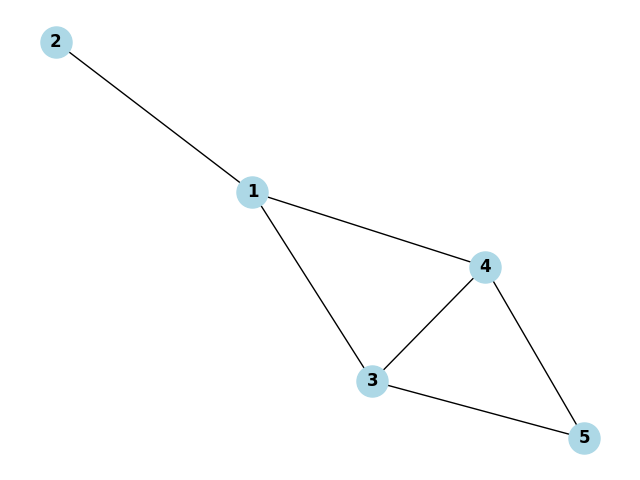
\includegraphics[width=0.65\textwidth]{grafo_instancia2.png}
            \caption{Grafo da instância 2 de entrada.}
            \label{fig:instancia2}
        \end{figure}

    \subsubsection{Instância 3}
        \begin{tcolorbox}[title=Arquivo de entrada para a instância 3, width=\linewidth, 
          fontupper=\ttfamily, 
          halign=flush left]
            10 \\
            0 1 0 0 0 1 1 0 0 0 \\
            1 0 0 0 1 0 1 0 1 0 \\
            0 0 0 1 0 0 1 1 1 1 \\
            0 0 1 0 1 1 0 1 1 0 \\
            0 1 0 1 0 0 0 0 0 1 \\
            1 0 0 1 0 0 0 0 0 0 \\
            1 1 1 0 0 0 0 0 0 1 \\
            0 0 1 1 0 0 0 0 0 1 \\
            0 1 1 1 0 0 0 0 0 0 \\
            0 0 1 0 1 0 1 1 0 0 \\
        \end{tcolorbox}

        \begin{tcolorbox}[title=Saída da instância 3, width=\linewidth, 
          fontupper=\ttfamily, 
          halign=flush left]
            [0, 0, 1, 0, 0, 0, 0, 1, 0, 1] \\
            Vértices presentes no clique: \\
            3 \\
            8 \\
            10 \\
            Tempo de execução: 0.000997 segundos \\
        \end{tcolorbox}

        \begin{figure}[H]
            \centering
            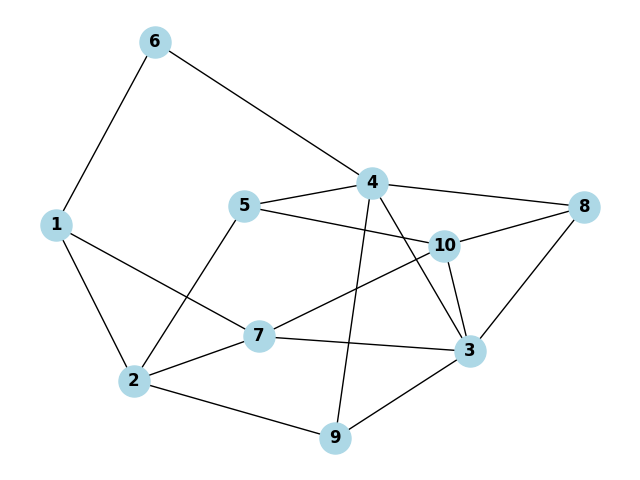
\includegraphics[width=0.65\textwidth]{grafo_instancia3.png}
            \caption{Grafo da instância 3 de entrada.}
            \label{fig:instancia3}
        \end{figure}
     
\clearpage
\section{Conjunto Independente}
    Para resolver o problema do Conjunto Independente (ou Conjunto Estável) por meio de uma redução polinomial ao problema do Clique, iremos usar a relação entre esses dois problemas. Sabemos que um conjunto independente de um grafo é equivalente a um clique no complemento desse grafo.\\
    
    \subsection{Lógica da função} \textbf{Passos para a solução}
    \begin{itemize}
        \item \textbf{Complemento do grafo:} O complemento de um grafo é um grafo onde as arestas que estavam presentes no grafo original são removidas e as arestas que não estavam presentes são adicionadas.
        \item \textbf{Redução:} Dado um grafo GGG, o problema do conjunto independente em GGG pode ser resolvido encontrandoo o clique máximo no complemento do grafo G'G'G'.
        \item \textbf{Aproveitar a implementação do clique:} Após calcular o complemento do grafo, aplicamos o algoritmo de clique já implementado.\\
    \end{itemize}


\subsection{Função geraComplemento}

O Código \ref{lst:cod1} apresenta a função que foi implementada para gerar o complemento do grafo.

\begin{lstlisting}[caption={Função que gera o complemento do grafo para o problema do conjunto independente},label={lst:cod1},language=Python]
def geraComplemento(problema):
    numVertices = problema[0][0]  # Numero de vertices (primeira linha da matriz)
    
    # Inicializa a matriz de complemento
    complemento = [[0] * numVertices for _ in range(numVertices)]
    
    # Preenche a matriz de complemento
    for i in range(numVertices):
        for j in range(numVertices):
            if i != j:  # Nao considerar a diagonal principal
                complemento[i][j] = 1 - problema[i + 1][j]
    
    # Adiciona o numero de vertices como a primeira linha da matriz de complemento
    complemento.insert(0, [numVertices])
    
    return complemento
 \end{lstlisting}
    A função recebe como parâmetro de entrada uma matriz de adjacência que representa o grafo original. A primeira linha da matriz contém o número de vértices do grafo, e as linhas subsequentes indicam a presença de arestas entre os vértices. Um valor 1 indica que há uma aresta entre dois vértices, e um valor 0 indica que não há aresta.
    \par \textbf{Passos da função: }
    \begin{itemize}
        \item \textbf{Captura o número de vértices:} O número de vértices do grafo é obtido da primeira linha da matriz problema. A linha problema[0][0] armazena essa informação.
        
        \item \textbf{Inicializa a matriz do complemento:} 
        \begin{verbatim}
        complemento = [[0] * numVertices for _ in range(numVertices)]
        \end{verbatim}
        Nessa parte a função cria uma nova matriz quadrada de dimensão numVertices * numVertices, inicialmente preenchida com zeros. Essa matriz será preenchida com informações do complemento do grafo.
        
        \item \textbf{Preenche a matriz de complemento:} 
        \begin{verbatim}
        for i in range(numVertices):
            for j in range(numVertices):
                if i != j:
                    complemento[i][j] = 1 - problema[i + 1][j]
        \end{verbatim}
        A função utiliza dois loops aninhados para percorrer todos os pares de vértices (i, j) do grafo e, para cada par, verifica se os vértices são diferentes. Isso é necessário porque um vértice não pode ser adjacente a si mesmo. Para os pares de vértices distintos, a função calcula o complemento da adjacência: se há uma arestas entre dois vértices no grafo original, o complemento remove essa aresta (1 vira 0), e se não há aresta, o complemento a adiciona (0 vira 1).

        \item \textbf{Adiciona o número de vértices como a primeira linha:} 
        \begin{verbatim}
            complemento.insert(0, [numVertices])
        \end{verbatim}
        Após gerar a matriz de adjacência do complemento, a função insere o número de vértices como primeira linha da matriz, para manter o mesmo formato da matriz original (onde a primeira linha sempre indica a quantidade de vértices).
    \end{itemize}
\subsection{Exemplos de instância do problema}
    \subsubsection{Instância 1}
        \begin{tcolorbox}[title=Arquivo de entrada para a instância 1, width=\linewidth, 
          fontupper=\ttfamily, 
          halign=flush left]
            9 \\
            0 0 1 0 0 0 0 0 0 \\
            0 0 1 0 0 0 0 0 0 \\
            1 1 0 1 1 0 0 0 0 \\
            0 0 1 0 0 0 1 0 0 \\
            0 0 1 0 0 1 0 1 0 \\
            0 0 0 0 1 0 0 0 0 \\
            0 0 0 1 0 0 0 1 1 \\
            0 0 0 0 1 0 1 0 1 \\
            0 0 0 0 0 0 1 1 0 \\
        \end{tcolorbox}

        \begin{tcolorbox}[title=Saída da instância 1, width=\linewidth, 
          fontupper=\ttfamily, 
          halign=flush left]
            Conjunto independente máximo: {1, 2, 4, 6, 9}\\
            Tempo de execução: 0.002493 segundos\\
        \end{tcolorbox}

        \begin{figure}[H]
            \centering
            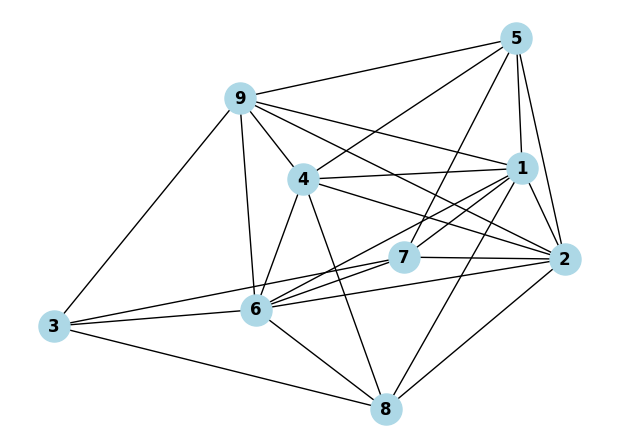
\includegraphics[width=0.65\textwidth]{conj_instancia1.png}
            \caption{Grafo complemento da instância 1 de entrada.}
            \label{fig:instancia1}
        \end{figure}

        \subsubsection{Instância 2}
        \begin{tcolorbox}[title=Arquivo de entrada para a instância 2, width=\linewidth, 
          fontupper=\ttfamily, 
          halign=flush left]
            5 \\
            0 1 1 1 0 \\
            1 0 0 0 0 \\
            0 1 0 1 1 \\
            1 0 1 0 1 \\
            0 0 1 1 0 \\
        \end{tcolorbox}

        \begin{tcolorbox}[title=Saída da instância 2, width=\linewidth, 
          fontupper=\ttfamily, 
          halign=flush left]
            Conjunto independente máximo: {1, 3, 5}
            Tempo de execução: 0.001508 segundos
        \end{tcolorbox}
        
        \begin{figure}[H]
            \centering
            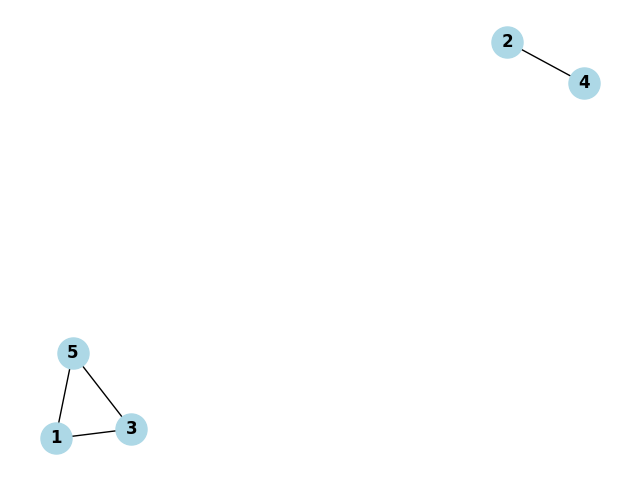
\includegraphics[width=0.65\textwidth]{conj_instancia2.png}
            \caption{Grafo complemento da instância 2 de entrada.}
            \label{fig:instancia1}
        \end{figure}
        
        \subsubsection{Instância 3}
        \begin{tcolorbox}[title=Arquivo de entrada para a instância 3, width=\linewidth, 
          fontupper=\ttfamily, 
          halign=flush left]
            10 \\
            0 1 0 0 0 1 1 0 0 0 \\
            1 0 0 0 1 0 1 0 1 0 \\
            0 0 0 1 0 0 1 1 1 1 \\
            0 0 1 0 1 1 0 1 1 0 \\
            0 1 0 1 0 0 0 0 0 1 \\
            1 0 0 1 0 0 0 0 0 0 \\
            1 1 1 0 0 0 0 0 0 1 \\
            0 0 1 1 0 0 0 0 0 1 \\
            0 1 1 1 0 0 0 0 0 0 \\
            0 0 1 0 1 0 1 1 0 0 \\
        \end{tcolorbox}

        \begin{tcolorbox}[title=Saída da instância 3, width=\linewidth, 
          fontupper=\ttfamily, 
          halign=flush left]
            Conjunto independente máximo: {5, 6, 7, 8, 9}\\
            Tempo de execução: 0.002523 segundos\\
        \end{tcolorbox}

        \begin{figure}[H]
            \centering
            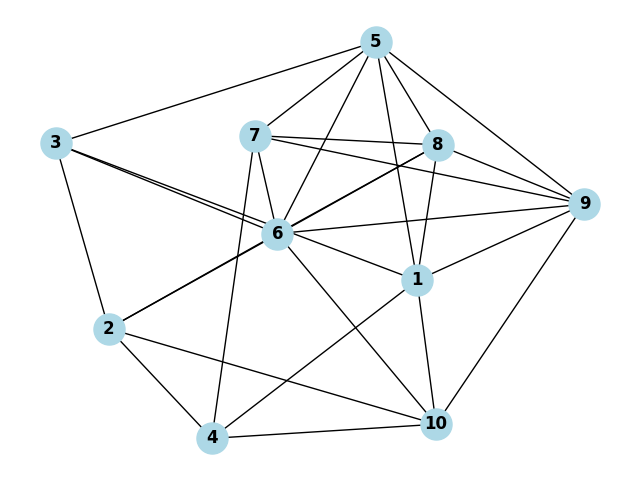
\includegraphics[width=0.65\textwidth]{conj_instancia3.png}
            \caption{Grafo complemento da instância 3 de entrada.}
            \label{fig:instancia1}
        \end{figure}

    

\clearpage
\section{Satisfabilidade}
    Para o problema da satisfabilidade (SAT), dada uma fórmula booleana na forma normal conjuntiva, é necessário encontrar, com \textit{backtracking}, algum resultado que satisfaça a mesma, ou, caso não seja possível satisfazer, informar a não possibilidade de satisfabilidade.

    Assim, para tal problema, podemos descrevê-lo da seguinte forma:
    \begin{itemize}
        \item \textbf{Variáveis para a solução:} \(X_1, \dots, X_n\), onde \(X_i\) indica o valor verdade para determinada variável do problema;
        \item \textbf{Domínio para as variáveis da solução:} \{False, True\}, indicando os valores lógicos falso e verdadeiro, respectivamente;
        \item \textbf{Restrições:} Todas as cláusulas devem resultar em verdadeiro
        \item \textbf{Objetivo:} Obter algum conjunto de valores do domínio para as variáveis de forma que todas as cláusulas sejam satisfeitas
    \end{itemize}

    \par Para a entrada do programa, é lido um arquivo onde a primeira linha indica uma quantidade N de variáveis e, as demais, indicam as cláusulas da fórmula. Cada cláusula é formada N valores inteiros, onde 1 representa a presença da variável na entrada, 0 indica a negação e -1 indica a ausência.

    \par A seguir temos o exemplo de entrada presente em um arquivo de entrada para a seguinte fórmula: \[(A \lor \neg B \lor C) \land (\neg A \lor B \lor D) \land (B \lor \neg C \lor \neg D) \land (\neg A \lor \neg B \lor D)\]

    \begin{tcolorbox}[title=Arquivo de entrada para a fórmula, width=\linewidth, 
      fontupper=\ttfamily, 
      halign=flush left]
        4 \\
        1 0 1 -1 \\
        0 1 -1 1 \\
        -1 1 0 0 \\
        0 0 -1 1
    \end{tcolorbox}
    
    \par Após a realização da leitura do arquivo, teremos uma lista de listas, onde a lista externa indica o problema como um todo e, cada lista interna, indica as clásulas.
    
    \begin{tcolorbox}[title=Entrada do programa para a fórmula fornecida, width=\linewidth, 
      fontupper=\ttfamily, 
      halign=flush left]
        [[1, 0, 1, -1], \newline [0, 1, -1, 1], \newline [-1, 1, 0, 0], \newline [0, 0, -1, 1]]
    \end{tcolorbox}

    \par Para o início da solução, é gerado um vetor \verb|solucao| com tamanho igual à quantidade de variáveis do problema SAT, onde cada posição é inicializada como nula.
    
    \par A seguir, é chamada a função \verb|backtrack|, passando como parâmetros \verb|solucao|, \verb|i|, indicando a última variável que teve valor atribuído, sendo que, neste primeiro momento será zero, e \verb|problema|, indicando a entrada lida.
    
    \par Na função \verb|backtrack|, primeiro verificamos se a \verb|solucao| é uma solução final, caso seja, retornamos o valor \verb|True| indicando que foi encontrada uma solução e encerramos todas as camadas recursivas retornando este valor.
    
    \par Caso a solução parcial não seja final, então identificamos os valores candidatos para a próxima variável a ser verificada e chamamos recursivamente a função \verb|backtrack|, onde os valores candidatos são pertencentes ao domínio do problema.

    \subsection{Verificar solução final}
    \par Para verificar se uma solução parcial é uma solução final, utilizamos a função \verb|verificar_solucao|, que recebe a instância do problema e a solução atual. 
    \par Primeiramente, verificamos se todos os valores da solução atual são diferentes de nulo, indicando se o \textit{bactracking} chegou a uma solução completa ou não. Caso uma variável seja nula, retornamos o valor falso, caso contrário, passaremos a verificar todas as cláusulas, onde, caso uma seja falsa, já retornamos que não é uma solução, pois não terá como satisfazer a fórmula desejada, e, ao satisfazer, retornamos que, de fato, é uma solução para o problema.

    \subsection{Gerar candidatos}
    \par Para a construção de candidatos realizada na função \verb|construir_candidatos|, recebemos a solução parcial, a variável atual que está sendo verificada, o problema e o domínio.
    \par Primeiramente, verificamos se todas as variáveis já tiveram valores atribuídos. Caso tenham, então retornamos uma lista vazia. Assim, não tendo candidatos, a função de \verb|backtrack| será finalizada para este ramo de opções.
    \par Agora, não retornando prematuramente, iremos atribuir, para a i-ésima variável, cada valor do domínio e verificar se, com o esse valor, a fórmula não terá a sua restrição violada.

    \par Dessa forma, com o valor atribuído e iterando sobre todas as cláusulas, verificamos se elas podem ser computáveis, ou seja, se todos o valor de todas as variáveis atribuidas até o momento estão presentes na mesma.
    \par No exemplo a seguir, verificamos que a cláusula não pode ser computada ainda, pois, com \verb|i = 3|, estamos verificando a viabilidade do valor \verb|True|. Todavia, com uma simples inspeção, verificamos que, até o momento, a cláusula é falsa. Mas como nada sabemos sobre as duas últimas variáveis, nada podemos afirmar, pois ela pode se tornar verdadeira ou continuar falsa. Logo, tal cláusula não pode ser computável no momento.
    \begin{tcolorbox}[width=\linewidth, fontupper=\ttfamily,  halign=flush left]
        Cláusula: 1 -1 0 0 1 \newline 
        Solução: [False, False, True, \_, \_] \newline
        i = 3
    \end{tcolorbox}

    \par Em formato de código, para realizar tal verificação, usamos a função \ref{lst:clausula_computavel}, onde verificamos se, da i-ésima variável em diante, todas têm valores -1, indicando que não estão presentes na fórmula. Assim, as próximas variáveis não impactarão no cálculo.


\begin{lstlisting}[caption={Verificando se cláusula é computável},label={lst:clausula_computavel}, language=Python]
def clausula_computavel(i, clausula, qtd_variaveis):  
    for j in range(i, qtd_variaveis):
        if clausula[j-1] == -1:
            return False
 \end{lstlisting}
    \par Vale ressaltar que, a presença ou ausência das variáveis anteriores ao valor \verb|i| não são necessárias verificações, pois garantimos que elas já foram atribuidas em passos anteriores do \textit{backtracking}.

    \par Agora, sabendo que a cláusula pode ser computável, verificamos se ela será satisfeita, para tanto, iteramos sobre todas as variáveis e verificamos o resultado ao final. A cláusula sendo verdadeira, verificamos a próxima, caso contrário, encerramos para tal valor do domínio e o retiramos da lista de candidatos, pois não será possível satisfazer a fórmula. 

    \subsection{Exemplos de instância}
    %%%%%%%%%%%%%%%%%%%%%%%%%%%%%%%%%%%%%%%%%%%%%%%%%%%%%%%%%%%%%%%%%%%%%%%%%%%%%%%%%%
    \subsubsection{Instância 1}
        \[(A \lor B \lor C) \land (A \lor \neg B) \land (B \lor \neg C) \land (\neg A \lor C) \land (\neg A \lor \neg B \lor \neg C)\]
        \begin{tcolorbox}[title=Entrada da instância 1, width=\linewidth, 
          fontupper=\ttfamily, 
          halign=flush left]
            3 \\ 
            1 1 1 \\
            1 0 -1 \\
            -1 1 0 \\
            0 -1 1 \\
            0 0 0 \\
        \end{tcolorbox}
        
        \begin{tcolorbox}[title=Saída da instância 1, width=\linewidth, fontupper=\ttfamily, halign=flush left]
            Solução não encontrada \\
            Tempo de execução: 0.000503 segundos \\  
        \end{tcolorbox}
    %%%%%%%%%%%%%%%%%%%%%%%%%%%%%%%%%%%%%%%%%%%%%%%%%%%%%%%%%%%%%%%%%%%%%%%%%%%%%%%%%%
    \subsubsection{Instância 2}
        \[(A \lor B \lor C) \land (\neg A \lor \neg B \lor \neg C)\]
        \begin{tcolorbox}[title=Entrada da instância 2, width=\linewidth, 
          fontupper=\ttfamily, 
          halign=flush left]
            3 \\
            1 1 1 \\
            0 0 0 \\
        \end{tcolorbox}
        
        \begin{tcolorbox}[title=Saída da instância 2, width=\linewidth, fontupper=\ttfamily, halign=flush left]
            Solução encontrada: [False, False, True] \\
            Tempo de execução: 0.000090 segundos   \\
        \end{tcolorbox}
    %%%%%%%%%%%%%%%%%%%%%%%%%%%%%%%%%%%%%%%%%%%%%%%%%%%%%%%%%%%%%%%%%%%%%%%%%%%%%%%%%%

    \subsubsection{Instância 3}
        \[(A \lor \neg B \lor C) \land (\neg A \lor B \lor D) \land (B \lor \neg C \lor \neg D) \land (\neg A \lor \neg B \lor D)\]
        \begin{tcolorbox}[title=Entrada da instância 3, width=\linewidth, fontupper=\ttfamily,  halign=flush left]
            4 \\
            1 0 1 -1 \\
            0 1 -1 1 \\
            -1 1 0 0 \\
            0 0 -1 1 \\

        \end{tcolorbox}
        \begin{tcolorbox}[title=Saída da instância 3, width=\linewidth, fontupper=\ttfamily, halign=flush left]
            Solução encontrada: [False, False, False, False] \\
            Tempo de execução: 0.000175 segundos
        \end{tcolorbox}

    %%%%%%%%%%%%%%%%%%%%%%%%%%%%%%%%%%%%%%%%%%%%%%%%%%%%%%%%%%%%%%%%%%%%%%%%%%%%%%%%%%
    \subsubsection{Instância 4}
    
        \[(\neg B \lor \neg C) \land (\neg A \lor C) \land (\neg A \lor B) \land (\neg B \lor \neg C) \land (A \lor C) \land (A \lor B)\]
        \begin{tcolorbox}[title=Entrada da instância 4, width=\linewidth, fontupper=\ttfamily,  halign=flush left]
            3 \\
            -1 0 0 \\
            0 -1 1 \\
            0 1 -1 \\
            -1 0 0 \\
            1 -1 1 \\
            1 1 -1 \\
        \end{tcolorbox}
        \begin{tcolorbox}[title=Saída da instância 4, width=\linewidth, fontupper=\ttfamily, halign=flush left]
            Solução não encontrada \\
            Tempo de execução: 0.000192 segundos
        \end{tcolorbox}

    %%%%%%%%%%%%%%%%%%%%%%%%%%%%%%%%%%%%%%%%%%%%%%%%%%%%%%%%%%%%%%%%%%%%%%%%%%%%%%%%%%

    \subsubsection{Instância 5}
        \[(A \lor B \lor C \lor D) \land (\neg A \lor \neg B \lor C) \land (A \lor \neg C \lor D) \land (\neg B \lor D)\]
        \begin{tcolorbox}[title=Entrada da instância 5, width=\linewidth, fontupper=\ttfamily,  halign=flush left]
            4 \\
            1 1 1 1 \\
            0 0 1 -1 \\
            1 -1 0 1 \\
            -1 0 -1 1 \\
        \end{tcolorbox}
        \begin{tcolorbox}[title=Saída da instância 5, width=\linewidth, fontupper=\ttfamily, halign=flush left]
            Solução encontrada: [False, False, False, True] \\
            Tempo de execução: 0.000134 segundos
        \end{tcolorbox}

    %%%%%%%%%%%%%%%%%%%%%%%%%%%%%%%%%%%%%%%%%%%%%%%%%%%%%%%%%%%%%%%%%%%%%%%%%%%%%%%%%%
    
    \subsubsection{Instância 6}
        \((A \lor B \lor C) \land (\neg A \lor \neg B \lor \neg C) \land (A \lor \neg B \lor D) \land (\neg A \lor B \lor \neg D) \land (A \lor \neg C \lor D) \land (\neg A \lor C \lor \neg D) \land (\neg A \lor \neg B \lor C \lor D) \land (A \lor B \lor \neg C \lor \neg D)\)
        \begin{tcolorbox}[title=Entrada da instância 6, width=\linewidth, fontupper=\ttfamily,  halign=flush left]
            4 \\
            1 1 1 -1 \\
            0 0 0 -1 \\
            1 0 -1 1 \\
            0 1 -1 0 \\
            1 -1 0 1 \\
            0 -1 1 0 \\
            0 0 1 1 \\
            1 1 0 0 \\
        \end{tcolorbox}
        \begin{tcolorbox}[title=Saída da instância 6, width=\linewidth, fontupper=\ttfamily, halign=flush left]
            Solução encontrada: [False, True, False, True] \\
            Tempo de execução: 0.000151 segundos
        \end{tcolorbox}
    
    %%%%%%%%%%%%%%%%%%%%%%%%%%%%%%%%%%%%%%%%%%%%%%%%%%%%%%%%%%%%%%%%%%%%%%%%%%%%%%%%%%
    \subsubsection{Instância 7}
        \((A \lor B \lor \neg C \lor D \lor E) \land (\neg A \lor \neg B \lor C \lor \neg E) \land (A \lor \neg C \lor \neg D \lor E) \land (\neg A \lor B \lor D) \land (C \lor \neg D \lor \neg E)\)
        \begin{tcolorbox}[title=Entrada da instância 7, width=\linewidth, fontupper=\ttfamily,  halign=flush left]
            5 \\
            1 1 0 1 1 \\
            0 0 1 -1 0 \\
            1 -1 0 0 1 \\
            0 1 -1 1 -1 \\
            -1 -1 1 0 0 \\
        \end{tcolorbox}
        \begin{tcolorbox}[title=Saída da instância 7, width=\linewidth, fontupper=\ttfamily, halign=flush left]
            Solução encontrada: [False, False, False, False, False] \\
            Tempo de execução: 0.000105 segundos
        \end{tcolorbox}
    %%%%%%%%%%%%%%%%%%%%%%%%%%%%%%%%%%%%%%%%%%%%%%%%%%%%%%%%%%%%%%%%%%%%%%%%%%%%%%%%%%
    \subsubsection{Instância 8}
        \((A \lor B \lor C) \land (\neg A \lor \neg B \lor \neg C) \land (A \lor \neg B \lor D) \land (\neg A \lor B \lor \neg D) \land (A \lor \neg C \lor D) \land (\neg A \lor C \lor \neg D) \land (\neg A \lor \neg B \lor C \lor D) \land (A \lor B \lor \neg C \lor \neg D)\)
        \begin{tcolorbox}[title=Entrada da instância 8, width=\linewidth, fontupper=\ttfamily,  halign=flush left]
            4 \\
            1 1 -1 -1 \\
            0 0 -1 -1 \\
            1 -1 1 -1 \\
            -1 -1 0 -1 \\
            0 1 0 1 \\
            -1 -1 -1 0 \\
        \end{tcolorbox}
        \begin{tcolorbox}[title=Saída da instância 8, width=\linewidth, fontupper=\ttfamily, halign=flush left]
            Solução encontrada: [True, False, False, False] \\
            Tempo de execução: 0.000208 segundos
        \end{tcolorbox}
    %%%%%%%%%%%%%%%%%%%%%%%%%%%%%%%%%%%%%%%%%%%%%%%%%%%%%%%%%%%%%%%%%%%%%%%%%%%%%%%%%% 
    \subsubsection{Instância 9}
        \[(\neg A \lor B) \land (A \lor \neg B) \land (A \lor B) \land (\neg A \lor \neg B)\]
        \begin{tcolorbox}[title=Entrada da instância 9, width=\linewidth, fontupper=\ttfamily,  halign=flush left]
            2 \\
            0 1 \\
            1 0 \\
            1 1 \\
            0 0 \\
        \end{tcolorbox}
        \begin{tcolorbox}[title=Saída da instância 9, width=\linewidth, fontupper=\ttfamily, halign=flush left]
            Solução não encontrada \\
            Tempo de execução: 0.000091 segundos
        \end{tcolorbox}
    %%%%%%%%%%%%%%%%%%%%%%%%%%%%%%%%%%%%%%%%%%%%%%%%%%%%%%%%%%%%%%%%%%%%%%%%%%%%%%%%%%
    \subsubsection{Instância 10}
        \[(\neg A )\]
        \begin{tcolorbox}[title=Entrada da instância 10, width=\linewidth, fontupper=\ttfamily,  halign=flush left]
            1 \\
            0 \\
        \end{tcolorbox}
        \begin{tcolorbox}[title=Saída da instância 10, width=\linewidth, fontupper=\ttfamily, halign=flush left]
            Solução encontrada: [False] \\
            Tempo de execução: 0.000102 segundos
        \end{tcolorbox}



\clearpage


\clearpage
\section{Considerações Finais}
    \par Com o fim do desenvolvimento do trabalho, desenvolvemos nossos conhecimentos sobre branch and bound, redução polinomial e backtracking ao colocar, na prática, os conhecimentos antes apresentados de forma teórica.

    \par Ademais, o trabalho também foi útil para relembrarmos conceitos da Teoria dos Grafos, como o fato de que o conjunto independente máximo poder ser calculado a partir do complemento de um grafo e executando o algoritmo do Clique Máximo para o mesmo.

\clearpage
\bibliographystyle{plainnat} % ou outro estilo compatível
\bibliography{refs}

\end{document}



\subsection{Incluindo figuras}

Primeiro você precisa fazer o upload do arquivo de imagem do seu computador usando o link de upload no menu da árvore de arquivos. Em seguida, use o comando \texttt{\textbackslash includegraphics} para incluí-lo em seu documento. Use o ambiente de figura e o comando de legenda para adicionar um número e uma legenda à sua figura. Veja o código da Figura~\ref{fig:frog} nesta seção para um exemplo.

\begin{figure}[!htb]
    \centering
    \includegraphics[width=0.3\textwidth]{frog.jpg}
    \caption{Este sapo foi carregado por meio do menu da árvore de arquivos.}
    \label{fig:frog}
\end{figure}

Observe que sua figura será automaticamente colocada no local mais apropriado para ela, dado o texto ao redor e levando em consideração outras figuras ou tabelas que possam estar próximas. Você pode saber mais sobre como adicionar imagens aos seus documentos neste artigo de ajuda em \href{https://www.overleaf.com/learn/how-to/Including_images_on_Overleaf}{incluindo imagens no Overleaf}.



\subsection{Incluindo tabelas}

Use os ambientes \texttt{\textbackslash table} e \texttt{\textbackslash tabular} para tabelas básicas --- veja Tabela~\ref{tab:widgets}, por exemplo. Para obter mais informações, consulte este artigo de ajuda em \href{https://www.overleaf.com/learn/latex/tables}{tabelas}.

\begin{table}[!htb]
    \centering
    \begin{tabular}{|l|r|}
        \hline\hline
        Item & Quantidade \\\hline
        Item 1 & 42 \\
        Item 2 & 13 \\\hline\hline
    \end{tabular}
    \caption{\label{tab:widgets}Exemplo de tabela.}
\end{table}

Você pode usar editores online como o \href{https://www.tablesgenerator.com/}{\textit{Tables Generator}} para criar as suas tabelas.

\subsection{Incluindo listas}

Você pode fazer listas com numeração automática \dots

\begin{enumerate}
    \item Item 1.
    \item Item 2.
\end{enumerate}
\dots ou marcadores \dots
\begin{itemize}
    \item Item 1.
    \item Item 2.
\end{itemize}

\subsection{Incluindo equações matemáticas}

\LaTeX{} é ótimo na composição de matemática. Seja $X_1, X_2, \ldots, X_n$ uma sequência de variáveis aleatórias independentes e identicamente distribuídas com $\text{E}[X_i] = \mu$ e $\text{Var}[X_i] = \sigma^2 <\infty$, e deixe
\[S_n = \frac{X_1 + X_2 + \cdots + X_n}{n}
       = \frac{1}{n}\sum_{i}^{n} X_i\]
denotar sua média. Então, à medida que $n$ se aproxima do infinito, as variáveis aleatórias $\sqrt{n}(S_n - \mu)$ convergem na distribuição para um $\mathcal{N}(0, \sigma^2)$ normal.

\subsection{Incluindo citações e lista de referências}

Você pode simplesmente enviar um \verb|.bib| arquivo contendo suas entradas BibTeX, criado com uma ferramenta como JabRef ou procurar no Google Scholar. Você pode então citar entradas dele, assim: \cite{greenwade93} (colocando \textbackslash cite\{codigo\_no\_refs.bib\}). Apenas lembre-se de especificar um estilo de bibliografia, bem como o nome do arquivo \verb|.bib|. Você pode encontrar um \href{https://www.overleaf.com/help/97-how-to-include-a-bibliography-using-bibtex}{vídeo tutorial aqui} para saber mais sobre o BibTeX.

\subsection{Incluindo fragmento de códigos}

O Código \ref{lst:cod1} apresenta um exemplo de código para a sequência de Fibonacci em C.

\begin{lstlisting}[caption={Exemplo de código para a sequência de Fibonacci.},label={lst:cod1},language=C]
#include <stdio.h>

int main() {
   /* comentario */
   int n, i, a = 0, b = 1, F;
   printf("Digite o numero de termos da sequencia de Fibonacci: ");
   scanf("%d", &n);
   printf("%d %d ", a, b);
   for (i = 0; i < n - 2; i++) {
     F = a + b;
     printf("%d ", F);
     a = b;
     b = F;
   } 
   printf("\n");
   return 0;
 }
 \end{lstlisting}